
\hspace*{0.6cm}Энэ бүлэгт системийн гурван үндсэн
давхарга (Фронтэнд давхарга, Бэкэнд давхарга, Өгөгдлийн давхарга) тус бүрийн загварчлал, хил
хязгаар, нэгдсэн зохиомжийн шийдвэрийг дэлгэрэнгүй авч үзнэ.

% ─────────────────────────────────────────────────────────────────────
\section{Архитектурын үндэслэл}

Энэхүү судалгааны ажлын хүрээнд МУИС-ийн дипломын ажлын удирдлагын системийг холимог технологийн микрофронтэнд архитектураар шийдвэрлэх туршилтын загварын дагуу боловсруулсан. Судалгааны гол зорилго нь уламжлалт Java Enterprise экосистемийн төлөөлөл болох Jakarta Server Faces 2.2 (JSF) суурьтай монолит орчныг, орчин үеийн React суурьтай микрофронтэндүүдтэй хэрхэн оновчтой хослуулж, технологийн шилжилтийг эрсдэл багатай гүйцэтгэж болохыг архитектурын түвшинд загварчлан харуулахад оршино.

\subsection{Тулгамдсан асуудал}

Системийн хост орчноор JSF-ийг сонгосон нь Enterprise түвшний байгууллагуудын систем- үүдэд түгээмэл тохиолддог архитектурын сорилтуудыг бодит орчинд турших зорилготой. JSF суурьтай монолит бүтэц нь дараах онцлог болон хязгаарлалтуудыг агуулдаг тул микро- фронтэнд шилжилтийг турших хамгийн тохиромжтой кейс болсон:

\begin{enumerate}
    \item Багасгах болон томруулах чадварын ялгаатай байдал: JVM heap дээрх HttpSession-д суурилсан JSF-ийн төлөв хадгалалт нь санах ойн өндөр хэрэглээ шаарддаг бол микрофронтэнд хэсэг нь клиент талд суурилсан, stateless шинж чанартай байх боломжийг олгоно.
    \item Технологийн ялгаатай байдлыг нэгтгэх (Heterogeneity): JSF-ийн сервер талын Request-Response мөчлөгийг, React-ийн Single Page Application (SPA) шинж чанартай хэрхэн зөрчилгүйгээр уялдаатай ажиллуулах нь архитектурын гол сорилт байв.
    \item Хөгжүүлэлтийн бие даасан байдал: Хост системийг хөндөхгүйгээр, шинээр нэмэгдэж буй модулиудыг орчин үеийн TypeScript, React экосистем дээр бие даан хөгжүүлж, нэгтгэх боломжийг судлах шаардлагатай байв.
\end{enumerate}

\subsection{Архитектурын стратегийн сонголт: Аажмын шилжилтийн хандлага}

Холимог архитектурыг хэрэгжүүлэхийн тулд Strangler Fig \cite{fowler_strangler} загварыг баримталсан. Энэхүү загвар нь JSF суурьтай монолит хост системийг хэвээр хадгалж, шинэ модулиудыг React микрофронтэнд хэлбэрээр түүний дотор аажмаар суулгах замаар нэгдмэл системийг бүрдүүлдэг.

Энэхүү хандлагыг сонгосон үндэслэлүүд:
\begin{itemize}
    \item Холимог орчныг дэмжих: JSF болон React технологиудыг нэг хэрэглэгчийн интерфэйс дотор зөрчилгүйгээр ажиллуулах бодит туршилт болох.
    \item Бизнесийн тасралтгүй байдал: Системийн ажиллагааг зогсоолгүйгээр, модуль бүрээр нь үе шаттайгаар шилжүүлэх боломжийг хангах.
\end{itemize}

\begin{table}[H]
    \centering
    \caption{Архитектурын стратегийн харьцуулалт (Туршилтын загвараар)}
    \label{tab:arch_strategy}
    \renewcommand{\arraystretch}{1}
    \begin{tabular}{lccc}
        \toprule
        \textbf{Шалгуур} & \textbf{Big Bang} & \textbf{In-place} & \textbf{Strangler Fig} \\
        \midrule
        Технологийн холимог байдал     & Боломжгүй  & Хязгаарлагдмал   & Бүрэн боломжтой \\
        Бизнесийн эрсдэл               & Өндөр      & Дунд             & Бага            \\
        Командын бие даасан байдал     & Бага       & Бага             & Өндөр           \\
        Модульчлагдсан байдал          & Дунд       & Бага             & Маш өндөр       \\
        Буцаалтын (Rollback) боломж    & Байхгүй    & Хэцүү            & Бүрэн           \\
        \bottomrule
    \end{tabular}
\end{table}
% ─────────────────────────────────────────────────────────────────────
\section{Микрофронтэнд архитектур}

Microfrontend (MFE) архитектур нь backend микросервисийн зарчмуудыг
frontend давхаргад хэрэглэх ойлголт бөгөөд Cam Jackson (2019)-ийн
тодорхойлсноор SPA-г бие даасан, тусдаа байршуулагдах
жижиг фронтэнд аппликейшнүүдийн нэгдэл гэж тодорхойлогдоно.

Энэхүү системд JSF Tomcat нь нэгдсэн хостыг
үүрэг гүйцэтгэж, React дээр суурилсан бие даасан модулиуд нь нийлүүлэгч MFE хэлбэрт ажиллана. Ажиллах үеийн интеграцийн стратегийг ашигласан нь интеграцийн цагт биш,
харин хөтчид ачааллагдах үед модулиуд динамик байдлаар холбогдоно
гэсэн утгатай бөгөөд энэ нь Дэлхийн тэргүүлэх MFE архитектурын загвар
юм \cite{mezzalira2021}.


\subsection{Strangler Fig үлгэр загварын хэрэгжүүлэлт}
Strangler Fig үлгэр загвар \cite{fowler2004} нь Австралийн чулуун инжир модны органик ургалтын хэлбэрээс санаа авсан архитектурын хандлага бөгөөд энэ нь хуучин системийг зогсоолгүйгээр, шинэ бүрэлдэхүүн хэсгүүдийг аажмаар нэгтгэн орлуулах боломжийг олгодог. Энэхүү судалгааны ажлын хүрээнд JSF суурьтай монолит бүтцийг "Legacy Proxy" буюу уламжлалт системийн загвар болгон ашиглаж, орчин үеийн React MFE-тэй хэрхэн зэрэгцэн ажиллах процессыг дараах үе шаттайгаар загварчлав:

\begin{enumerate}
	\item Identify (Жижиглэн хуваалт): Монолит архитектураас бие даасан байдлаар тусгаарлаж болох бизнесийн логик болон домейны хил хязгаарыг тодорхойлох шат юм. Дипломын ажлын удирдлагын системийн хүрээнд нэвтрэлт, оюутан, багш болон захиргааны хэсгүүдийг тусдаа контекст болгон тодорхойлсон.
	\item Strangle (Интеграци): Сонгосон функциональ хэсгүүдийг React MFE хэлбэрт хөгжүүлж, JSF хост доторх тусгай цэгүүдэд (Injection points) суулгасан. Энэ нь технологийн ялгаатай хоёр орчин нэг хэрэглэгчийн интерфейс дотор зөрчилгүй ажиллах холимог үе шат юм.
	\item Transform/Transition (Шилжилт): Бүх модулиудыг MFE хэлбэрт шилжүүлснээр систем бүрэн микрофронтэнд архитектурт шилжих боломж бүрдэнэ.
\end{enumerate}

\textbf{Судалгааны хязгаарлалт ба хамрах хүрээ:} Энэхүү судалгаа нь Strangler Fig үлгэр загварын \textbf{Strangle} буюу холимог орчинд технологиудыг нэгтгэн ажиллуулах үе шатыг голлон анхаарсан. JSF хостыг бүрэн устгаж, 100\% бие даасан SPA (Single Page Application) болгон хувиргах эцсийн шатыг судалгааны хамрах хүрээнээс гадуур буюу ирээдүйд хийгдэх ажлын хэсэгт үлдээв. Ингэснээр системд эрсдэлгүй шилжилт хийх боломжтойг архитектурын хувьд баталсан болно.
\subsection{MFE модулиудын зохион байгуулалт}

Системийн архитектурыг Eric Evans \cite{evans2003}-ийн тодорхойлсон Хязгаарлагдсан контекст (Bounded Context) зарчмын дагуу хуваасан. Ингэснээр модуль бүр өөрийн домейны хил хязгаар, өгөгдлийн загвар болон бизнесийн хариуцлагыг бие даан хариуцах боломж бүрдсэн. Туршилтын хүрээнд дараах долоон бие даасан MFE модулийг загварчлан хэрэгжүүлэв.

\begin{longtable}{p{3.5cm} p{12.5cm}}
\caption{MFE модулиудын зохион байгуулалт} \label{tab:mfe} \\
\toprule
\textbf{MFE модуль} & \textbf{Архитектурын үүрэг ба хариуцлага} \\ 
\midrule
\endfirsthead
\toprule
\textbf{MFE модуль} & \textbf{Архитектурын үүрэг ба хариуцлага} (үргэлжлэл) \\ 
\midrule
\endhead
\bottomrule
\endfoot

\textbf{host-jsf} & Микрофронтэндүүдийг нэгдсэн нэг интерфейст нэгтгэх үндсэн бүрхүүл үүргийг гүйцэтгэнэ. Үүнд:
\begin{itemize}
\item Глобал чиглүүлэлт болон нэвтрэх эрхийн төвлөрсөн хяналт;
\item Системийн нэгдсэн бүтэц болон навигацийн удирдлага;
\item Бие даасан MFE модулиудыг хэрэгцээт цагт нь динамикаар дуудаж ажиллуулах интеграцчлал.
\end{itemize} \\ \addlinespace

\textbf{module-auth} & Хэрэглэгчийг таних, баталгаажуулах болон системийн сессийг эхлүүлэх урсгалыг хариуцна. Аюулгүй байдлын үүднээс бусад модулиудаас хамааралгүй, тусгаарлагдсан контекстэд ажиллахаар загварчлагдсан. \\ \addlinespace

\textbf{module-student} & Оюутанд зориулсан бизнесийн бүх логикийг агуулна. Үүнд сэдэв сонгохоос эхлээд эцсийн хамгаалалт хүртэлх амьдралын мөчлөгийг удирдах бөгөөд бодит цагийн мэдэгдлийн сервистэй уялдаж ажиллана. \\ \addlinespace

\textbf{module-teacher} & Багшийн зүгээс хийгдэх хяналт, үнэлгээний үйлдлүүдийг хариуцна. Оюутны явцыг удирдах, зөвлөгөө өгөх болон өөрийн удирдаж буй ажлуудын нэгдсэн хяналтын самбарыг ажиллуулна. \\ \addlinespace

\textbf{module-admin} & Системийн суурь тохиргоо, тэнхимийн бүтэц, хэрэглэгчдийн эрх болон комисс хуваарилах зэрэг системийн түвшний зохицуулалтыг хариуцна. \\ \addlinespace

\textbf{shared-ui-module} & Системийн харагдац, дизайны нэгдмэл байдлыг хангах зорилготой. Бүх MFE-д ашиглагдах UI бүрэлдэхүүнүүдийг нэгтгэн хадгалж, системийн гүйцэтгэлийг оновчтой болгох үүднээс дундын нөөцийг хуваалцах (Shared resource) бодлогоор ажиллана. \\ \addlinespace
\end{longtable}

\begin{figure}[H]
\centering
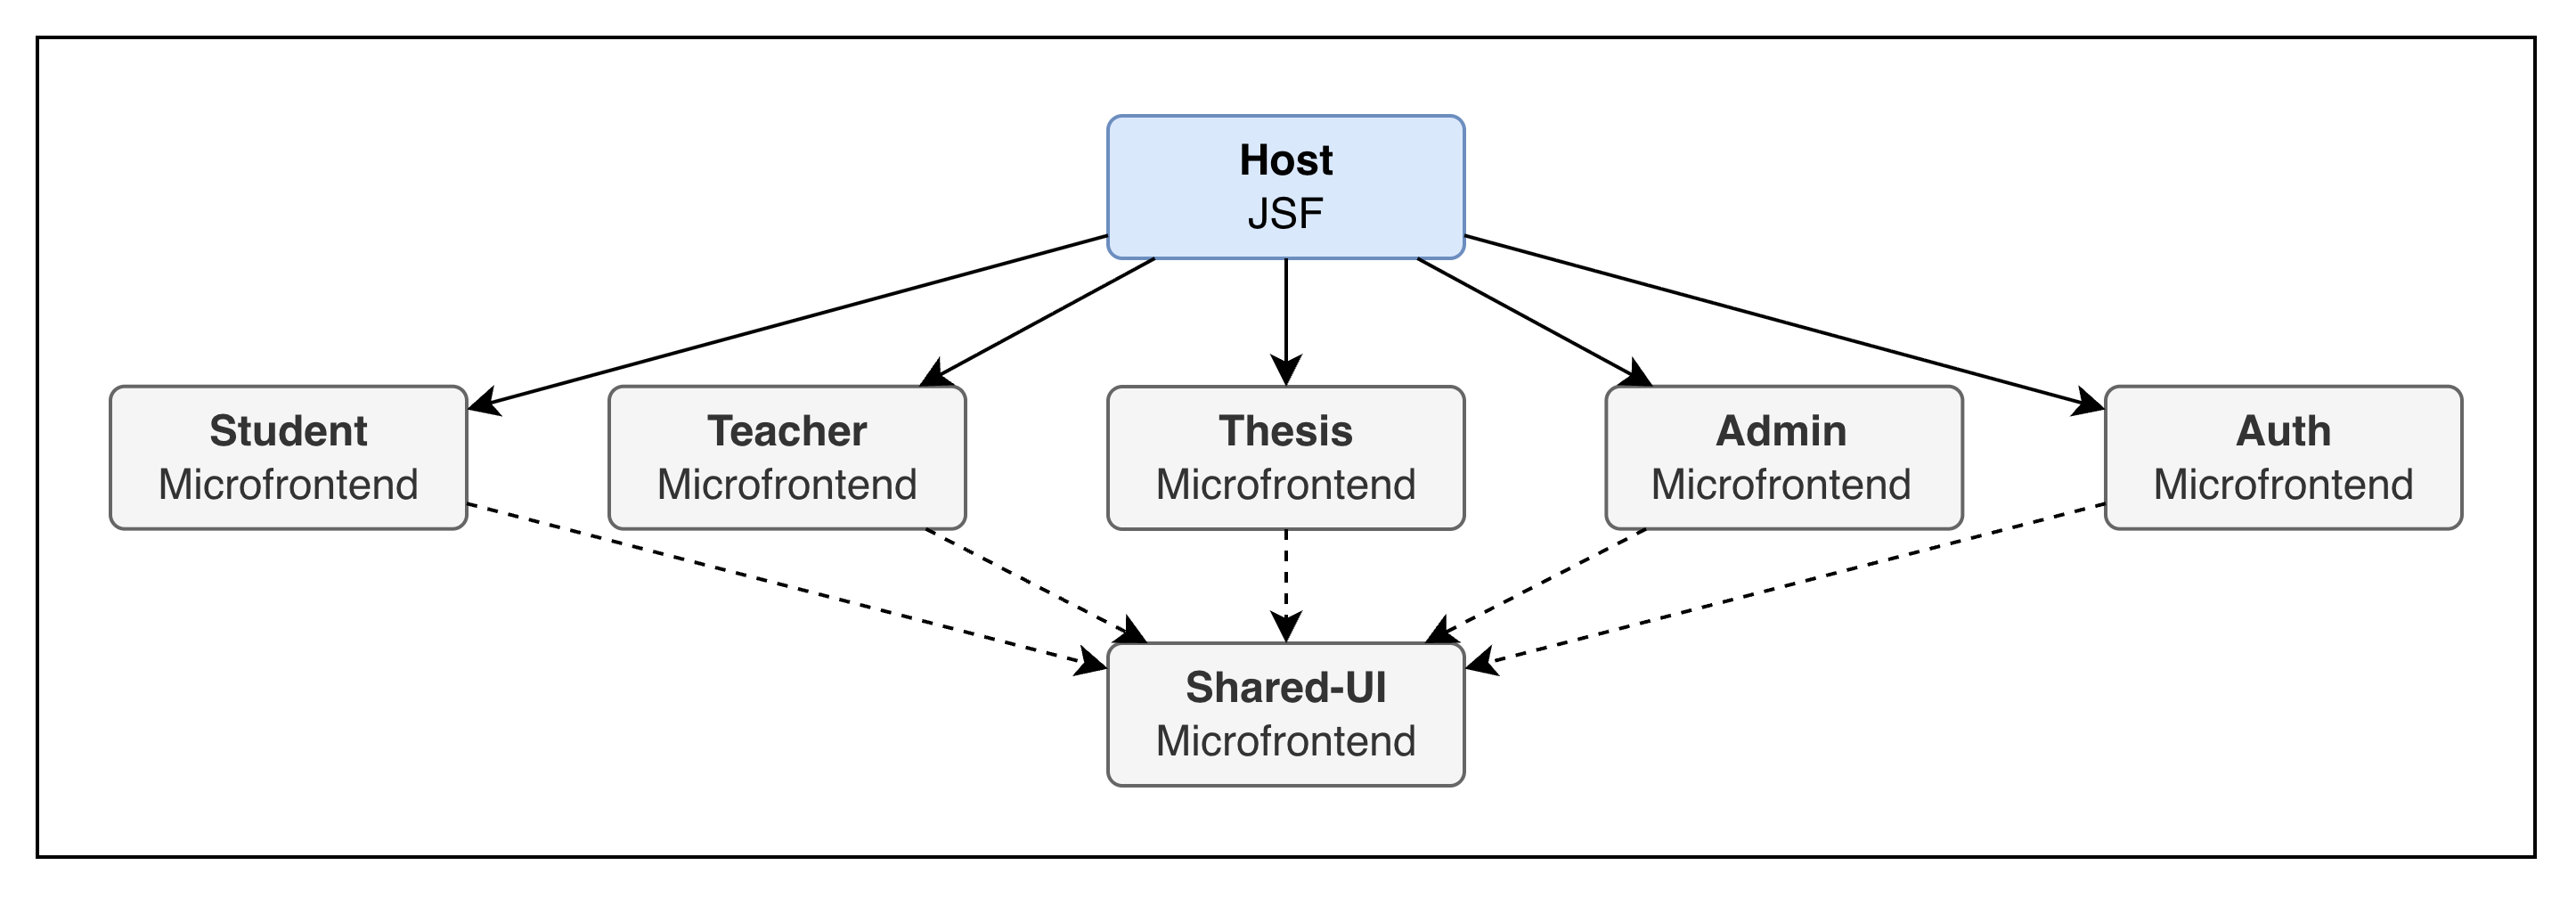
\includegraphics[width=16cm]{images/frontend.png}
\caption{Микрофронтэндүүд хоорондын харилцаа}
\label{fig:frontend}
\end{figure}

\subsection{Ажиллах үеийн интеграци}

MFE интеграцийн арга нь гурван ангилалд хуваагдана: Build-time
Integration (угсралтын үеийн), Server-side Integration (сервер
талын) болон Runtime Integration (ажиллах үеийн). Тус
системд Ажиллах үеийн интеграци сонгосны шалтгаан нь:

\begin{itemize}
  \item Угсралтын үеийн интеграци нь бие даасан байршуулалтыг зөвшөөрдөггүй,
    нэг модуль өөрчлөгдөх бүрт бүгдийг дахин build хийх шаардлагатай болно.
  \item Сервер талын интеграци нь JSF-ийн request-response
    мөчлөгтэй зөрчилдөж, нарийн тохиргоо шаардана.
  \item Ажиллах үеийн интеграци нь Vite Module Federation хэрэгслийн
    тусламжтайгаар хөтчид \texttt{remoteEntry.js}-г динамикаар татаж, зөвхөн
    шаардлагатай модулийг ачаалах ``lazy loading'' зарчмаар ажиллах
    боломжийг олгодог.
\end{itemize}

Ажиллах үеийн интеграцийн загварт \texttt{remoteEntry.js} нь Remote MFE-ийн
манифест үүрэг гүйцэтгэж, Host нь энэ файлыг
ачаалснаар тухайн MFE-ийн экспортлосон бүрэлдэхүүнүүдийн мэдрэх зам
(resolution path)-ийг олж авдаг.

\section{Микросервис Архитектур}
Бэкенд системийн архитектур нь Sam Newman \cite{newman2019}-ийн тодорхойлсон микросервисийн зарчмууд болон Eric Evans \cite{evans2003}-ийн Домейнд Суурилсан Зохиомж (Domain-Driven Design) аргачлалд тулгуурлан хийгдсэн. Системийн функцийг бие даасан сервист хуваахдаа дараах хоёр үндсэн шалгуурыг баримтлав:

\begin{enumerate}
\item Хязгаарлагдсан Контекст: Домэйны мэдлэгийн хилийн зааг болон бизнесийн хариуцлагын дагуу логик хуваалт хийх.
\item Бие даасан масштаблах чадвар: Өндөр ачаалал авах магадлалтай болон бизнесийн чухал логик агуулсан хэсгүүдийг тусгаарлах замаар системийн уян хатан байдлыг хангах.
\end{enumerate}

\subsection{Микросервисийн архитектурын үүрэг}
Микросервисүүдийн зохион байгуулалт нь системийн бизнесийн логикийг тусгаарлах, өгөгдлийн бүтцийг оновчтой болгох, болон үйл ажиллагааны ачааллыг тэнцвэржүүлэхэд чиглэсэн. Хүснэгт \ref{tab:ms}-т микросервисүүдийн архитектурын үүрэг болон домэйн контекстын товч танилцуулга өгөгдсөн.



\begin{longtable}{p{3.5cm} p{12.5cm}}
\caption{Микросервисүүдийн зохион байгуулалт} \label{tab:ms} \\
\toprule
\textbf{Микросервис} & \textbf{Архитектурын үүрэг ба Домэйн контекст} \\ 
\midrule
\endfirsthead
\toprule
\textbf{Микросервис} & \textbf{Архитектурын үүрэг ба Домэйн контекст} (үргэлжлэл) \\ 
\midrule
\endhead
\bottomrule
\endfoot
\textbf{auth-service} & Системийн аюулгүй байдлын төвлөрсөн цэг. Хэрэглэгчийг таних, баталгаажуулах болон эрх олгох (IAM) логикийг хариуцна. \\ \addlinespace

\textbf{user-service} & Оюутан, багш, ажилтны хувийн мэдээлэл, харьяалагдах нэгж болон холбоо барих мэдээллийн нэгдсэн сан. \\ \addlinespace

\textbf{topic-service} & Дипломын ажлын сэдэв зарлах, хүсэлт авах, багш оюутны хослолыг баталгаажуулах логикийг тусгаарлан удирдана. \\ \addlinespace

\textbf{thesis-service} & Дипломын ажлын мета өгөгдөл, баримт бичгийн хувилбарчлал болон файлын хадгалах сангийн интеграцчлалыг хариуцна. \\ \addlinespace

\textbf{workflow-service} & Дипломын ажлын явцын төлөвийн шилжилтийг хянаж, бизнес процессын дарааллыг баталгаажуулна. \\ \addlinespace

\textbf{evaluation-service} & Комиссын гишүүд болон удирдагчийн зүгээс өгөх чанарын үнэлгээ, шүүмж болон санал хүсэлтийн логикийг агуулна. \\ \addlinespace

\textbf{grading-service} & Үнэлгээнүүдэд суурилан эцсийн оноог алгоритмын дагуу бодох, дүнгийн бүртгэл үүсгэх үүрэгтэй. \\ \addlinespace

\textbf{committee-service} & Хамгаалалтын комиссын бүрэлдэхүүн, тов болон зохион байгуулалтын логикийг хариуцна. \\ \addlinespace

\textbf{analytic-service} & Системийн дата дээр дүн шинжилгээ хийж, оюутнуудын явц, багш нарын ачаалал зэрэг статистик үзүүлэлтүүдийг боловсруулна. \\ \addlinespace

\textbf{report-service} & Системээс шаардлагатай албан ёсны бичиг баримт, протокол, дүнгийн жагсаалтыг файл хэлбэрээр үүсгэн гаргана. \\ \addlinespace

\textbf{notification-service} & Систем доторх мэдэгдэл, бодит цагийн мэдээллийг түгээх үүрэг бүхий туслах сервис. \\ \addlinespace

\textbf{API Gateway} & Гадаад хүсэлтийг хүлээн авч, JWT шалгалт болон чиглүүлэлт хийх замаар дотоод сервисүүдийг хамгаалах үүрэгтэй. \\ \addlinespace
\end{longtable}

% \section{Микросервис Архитектур}

% Backend-ийн архитектурын загварчлал нь Sam Newman \cite{newman2019building}-ийн
% ``Building Microservices'' болон Eric Evans \cite{evans2003domain}-ийн Domain-Driven
% Design зарчмуудад тулгуурлан хийгдсэн. Монолит backend нь ``Сервис бүр бие даан байршуулагдаж, нэг бизнесийн чадварыг хариуцна''
% гэсэн микросервисийн үндсэн зарчмын дагуу хуваагдсан. Хуваах шалгуур нь: нэгдүгээрт,
% Хязгаарлагдсан контекст (Bounded Context) буюу домейны мэдлэгийн
% хил хязгаар; хоёрдугаарт, Бизнесийн ажлын хэмжээний ялгаа, тухайлбал зарим
% сервис нь өндөр ачааллыг дааж чаддаг байх шаардлагатай бол зарим нь
% тийм ч их хэрэгцээгүй байдаг.

% \begin{figure}[H]
%     \centering
%     \includegraphics[width=14cm]
% 		% {fig_backend_microservices_overview.png}
% 		{images/backend.png}
%     \caption{Микросервис архитектурын шийдэл}
%     \label{fig:backend_overview}
% \end{figure}

% \subsection{Микросервисүүдийн Тодорхойлолт}

% \begin{longtable}{p{3.5cm} p{12.5cm}}
% \caption{Микросервисүүдийн зохион байгуулалт} \label{tab:ms} \\
% \toprule
% \textbf{Микросервис} & \textbf{Тодорхойлолт} \\ 
% \midrule
% \endfirsthead
% \toprule
% \textbf{Микро} & \textbf{Тодорхойлолт} (үргэлжлэл) \\ 
% \midrule
% \endhead
% \bottomrule
% \endfoot

% \textbf{auth-service} & Хэрэглэгчийн нэвтрэлт, JWT токен үүсгэх, нэвтрэлтийн оролдлого
% хянах, нууц үг сэргээх дараалал нь энэ сервисийн цөм хариуцлага юм.
% Auth-service нь \texttt{num\_auth-main} багцын дор байрладаг бөгөөд
% дотроо гурван дэд сервис агуулна: \texttt{auth-service} (нэвтрэлтийн
% цөм), \texttt{authorization-service} (эрхийн удирдлага),
% \texttt{user\_detail\_register} (хэрэглэгчийн дэлгэрэнгүй бүртгэл).

% JWT-ийн загвар нь Stateless буюу ``Claims суурилсан'' загвар бөгөөд
% токен нь \texttt{\{sisiId, roles, iat, exp\}} мэдэгдлийг агуулна.
% Токений хэрэглэнгийн хугацаа 24 цаг байхаар тохируулагдсан бөгөөд
% Refresh Token механизмийг нэмэлтээр дэмжнэ. \\ \addlinespace
% \textbf{user\_service} & Хэрэглэгчийн профайлын бүрэн мэдрэх хариуцлагыг хүлээнэ: оюутан,
% багш, хорооны гишүүн, хэлтсийн мэдээлэл. Auth-service нь зөвхөн
% нэвтрэлтийн мэдлэгтэй (\texttt{sisiId}, нууц үг) харьцуулбал
% user\_service нь дэлгэрэнгүй профайлын \textbf{единственный эх сурвалж}
% (Single Source of Truth) болно. Сервисийн endpoints нь
% \texttt{/api/users/students}, \texttt{/api/users/teachers},
% \texttt{/api/users/by-email} зэрэг болно. \\ \addlinespace
% \textbf{topic\_service} & Дипломын ажлын сэдвийн санд хариуцлагатай: сэдэв зарлах, хүсэлт
% хүлээн авах, оюутан-багш хосолт батлах. Энэ сервис нь
% \texttt{thesis\_service}-тэй нягт холбоотой боловч тусгаарлагдсан
% байдаг~--- сэдвийн амьдралын мөчлөг нь дипломын ажлын амьдралын
% мөчлөгтэй ялгаатай.
% \\ \addlinespace
% \textbf{thesis\_service} & Дипломын ажлын үндсэн мета мэдээллийг хадгалах, хувилбар удирдах,
% баримт бичгийн хавсаргалт зохицуулах. Дипломын ажлын нэр, хаяг, хар
% тэмдэглэл, файлын байршлын мета дата энд хадгалагдана. Файлын биет
% агуулга нь object storage (эсвэл локал файлын систем)-д хадгалагдаж,
% thesis\_service нь зөвхөн pointer хадгалдаг. \\ \addlinespace
% \textbf{workflow\_service} & Дипломын ажлын амьдралын мөчлөгийн статус шилжилтийг удирдана.
% State Machine загварт суурилсан бөгөөд төлөвүүд нь:
% \texttt{DRAFT → SUBMITTED → UNDER\_REVIEW → REVISION\_REQUESTED →
% APPROVED → DEFENSE\_SCHEDULED → DEFENDED → ARCHIVED}.
% Шилжилт бүр нь хугацааны тэмдэглэл, хариуцлагатай хэрэглэгч,
% тайлбарын бичлэгийг агуулна. \\ \addlinespace
% \textbf{evaluation\_service} & Комиссын гишүүн бүрийн дүгнэлтийг хүлээн авч, интеграцийн тооцоолол
% хийн, эцсийн дүн гаргах. Дүн гаргах алгоритм нь тохируулгатай
% (configurable) байхаар загварчлагдсан~--- жишилтийн жин, нийт онооны хязгаар гэх мэт. \\ \addlinespace
% \textbf{committee\_service} & Хэлэлцүүлгийн комиссын бүрэлдэхүүн тогтоох, хяналтын хуваарь гаргах, комиссын гишүүдэд мэдэгдэл илгээх. Энэ сервис нь \texttt{user\_service}-аас гишүүдийн мэдээлэл авч, \texttt{notification\_service}-тэй хамтарч мэдэгдэл явуулна. \\ \addlinespace
% \textbf{analytic\_service}
% \textbf{grading\_service}
% \textbf{report\_service}
% \textbf{notification\_service}
% \textbf{API Gateway} & Нэгдсэн нэвтрэх цэг (Single Entry Point) үүрэг гүйцэтгэж, гадаад хүсэлт бүрийг хүлээн авч, JWT шалгаж, тохирох upstream сервис рүү дамжуулна (proxy/reverse proxy). Rate limiting, request logging, CORS хяналт нь gateway давхаргад хэрэгжинэ тул backend сервис тус бүр энэ логикийг давтан хэрэгжүүлэх шаардлагагүй болно. \\ \addlinespace
% \end{longtable}

% \begin{table}[H]
%     \centering
%     \caption{Backend микросервисүүдийн порт болон хариуцлагын хуваарь}
%     \label{tab:service_ports}
%     \renewcommand{\arraystretch}{0.7}
%     \begin{tabular}{llll}
%         \toprule
%         \textbf{Сервис} & \textbf{Порт} & \textbf{Технологи} & \textbf{Гол хариуцлага} \\
%         \midrule
%         auth-service         & 8887 & Spring Boot  & JWT үүсгэх, нэвтрэлт \\
%         user\_service        & 8086 & Spring WebFlux & Хэрэглэгчийн профайл \\
%         topic\_service       & 8081 & Spring WebFlux & Сэдвийн удирдлага \\
%         thesis\_service      & 8083 & Spring WebFlux & Дипломын ажлын мета \\
%         workflow\_service    & 8084 & Spring WebFlux & Статус шилжилт \\
%         evaluation\_service  & 8085 & Spring WebFlux & Дүгнэлт, үнэлгээ \\
%         committee\_service   & 8082 & Spring WebFlux & Комиссын удирдлага \\
%         Tomcat (JSF+MFE)     & 8080 & Apache Tomcat  & Host, static file serve \\
%         \bottomrule
%     \end{tabular}
% \end{table}

\subsection{Сервис хоорондын харилцаа}
Микросервисүүд хоорондоо мэдээлэл солилцох, үйл ажиллагаагаа уялдуулахдаа системийн гүйцэтгэл болон найдвартай байдлыг хангах үүднээс дараах хоёр үндсэн үлгэр загварыгхослуулан ашиглахаар загварчлав.

\begin{enumerate}
\item \textbf{Синхрон харилцаа:} Бодит хугацааны хариу шаардлагатай, хүсэлт-хариултын дараалалд үндэслэсэн үйлдлүүдэд HTTP/REST протоколыг ашиглана. Системийн найдвартай байдлыг хангах зорилгоор Circuit Breaker үлгэр загварыг нэвтрүүлж, аль нэг сервисийн саатал нь бусад сервисүүдэд нөлөөлөхөөс сэргийлнэ.

\item \textbf{Асинхрон харилцаа:} Цаг хугацааны хамаарал, системийн хүлээлтийг багасгах зорилгоор үзэгдэлд суурилсан загварыг ашиглана. Мэдэгдэл илгээх, аудит бүртгэл хөтлөх зэрэг үйлдлүүд нь энэ загварт хамаарна. Архитектурын багасгах болон томруулах боломжтой байдлыг нэмэгдүүлэх үүднээс Message Broker (Apache Kafka, RabbitMQ) ашиглахаар сонгосон.
\end{enumerate}

\begin{figure}[H]
\centering
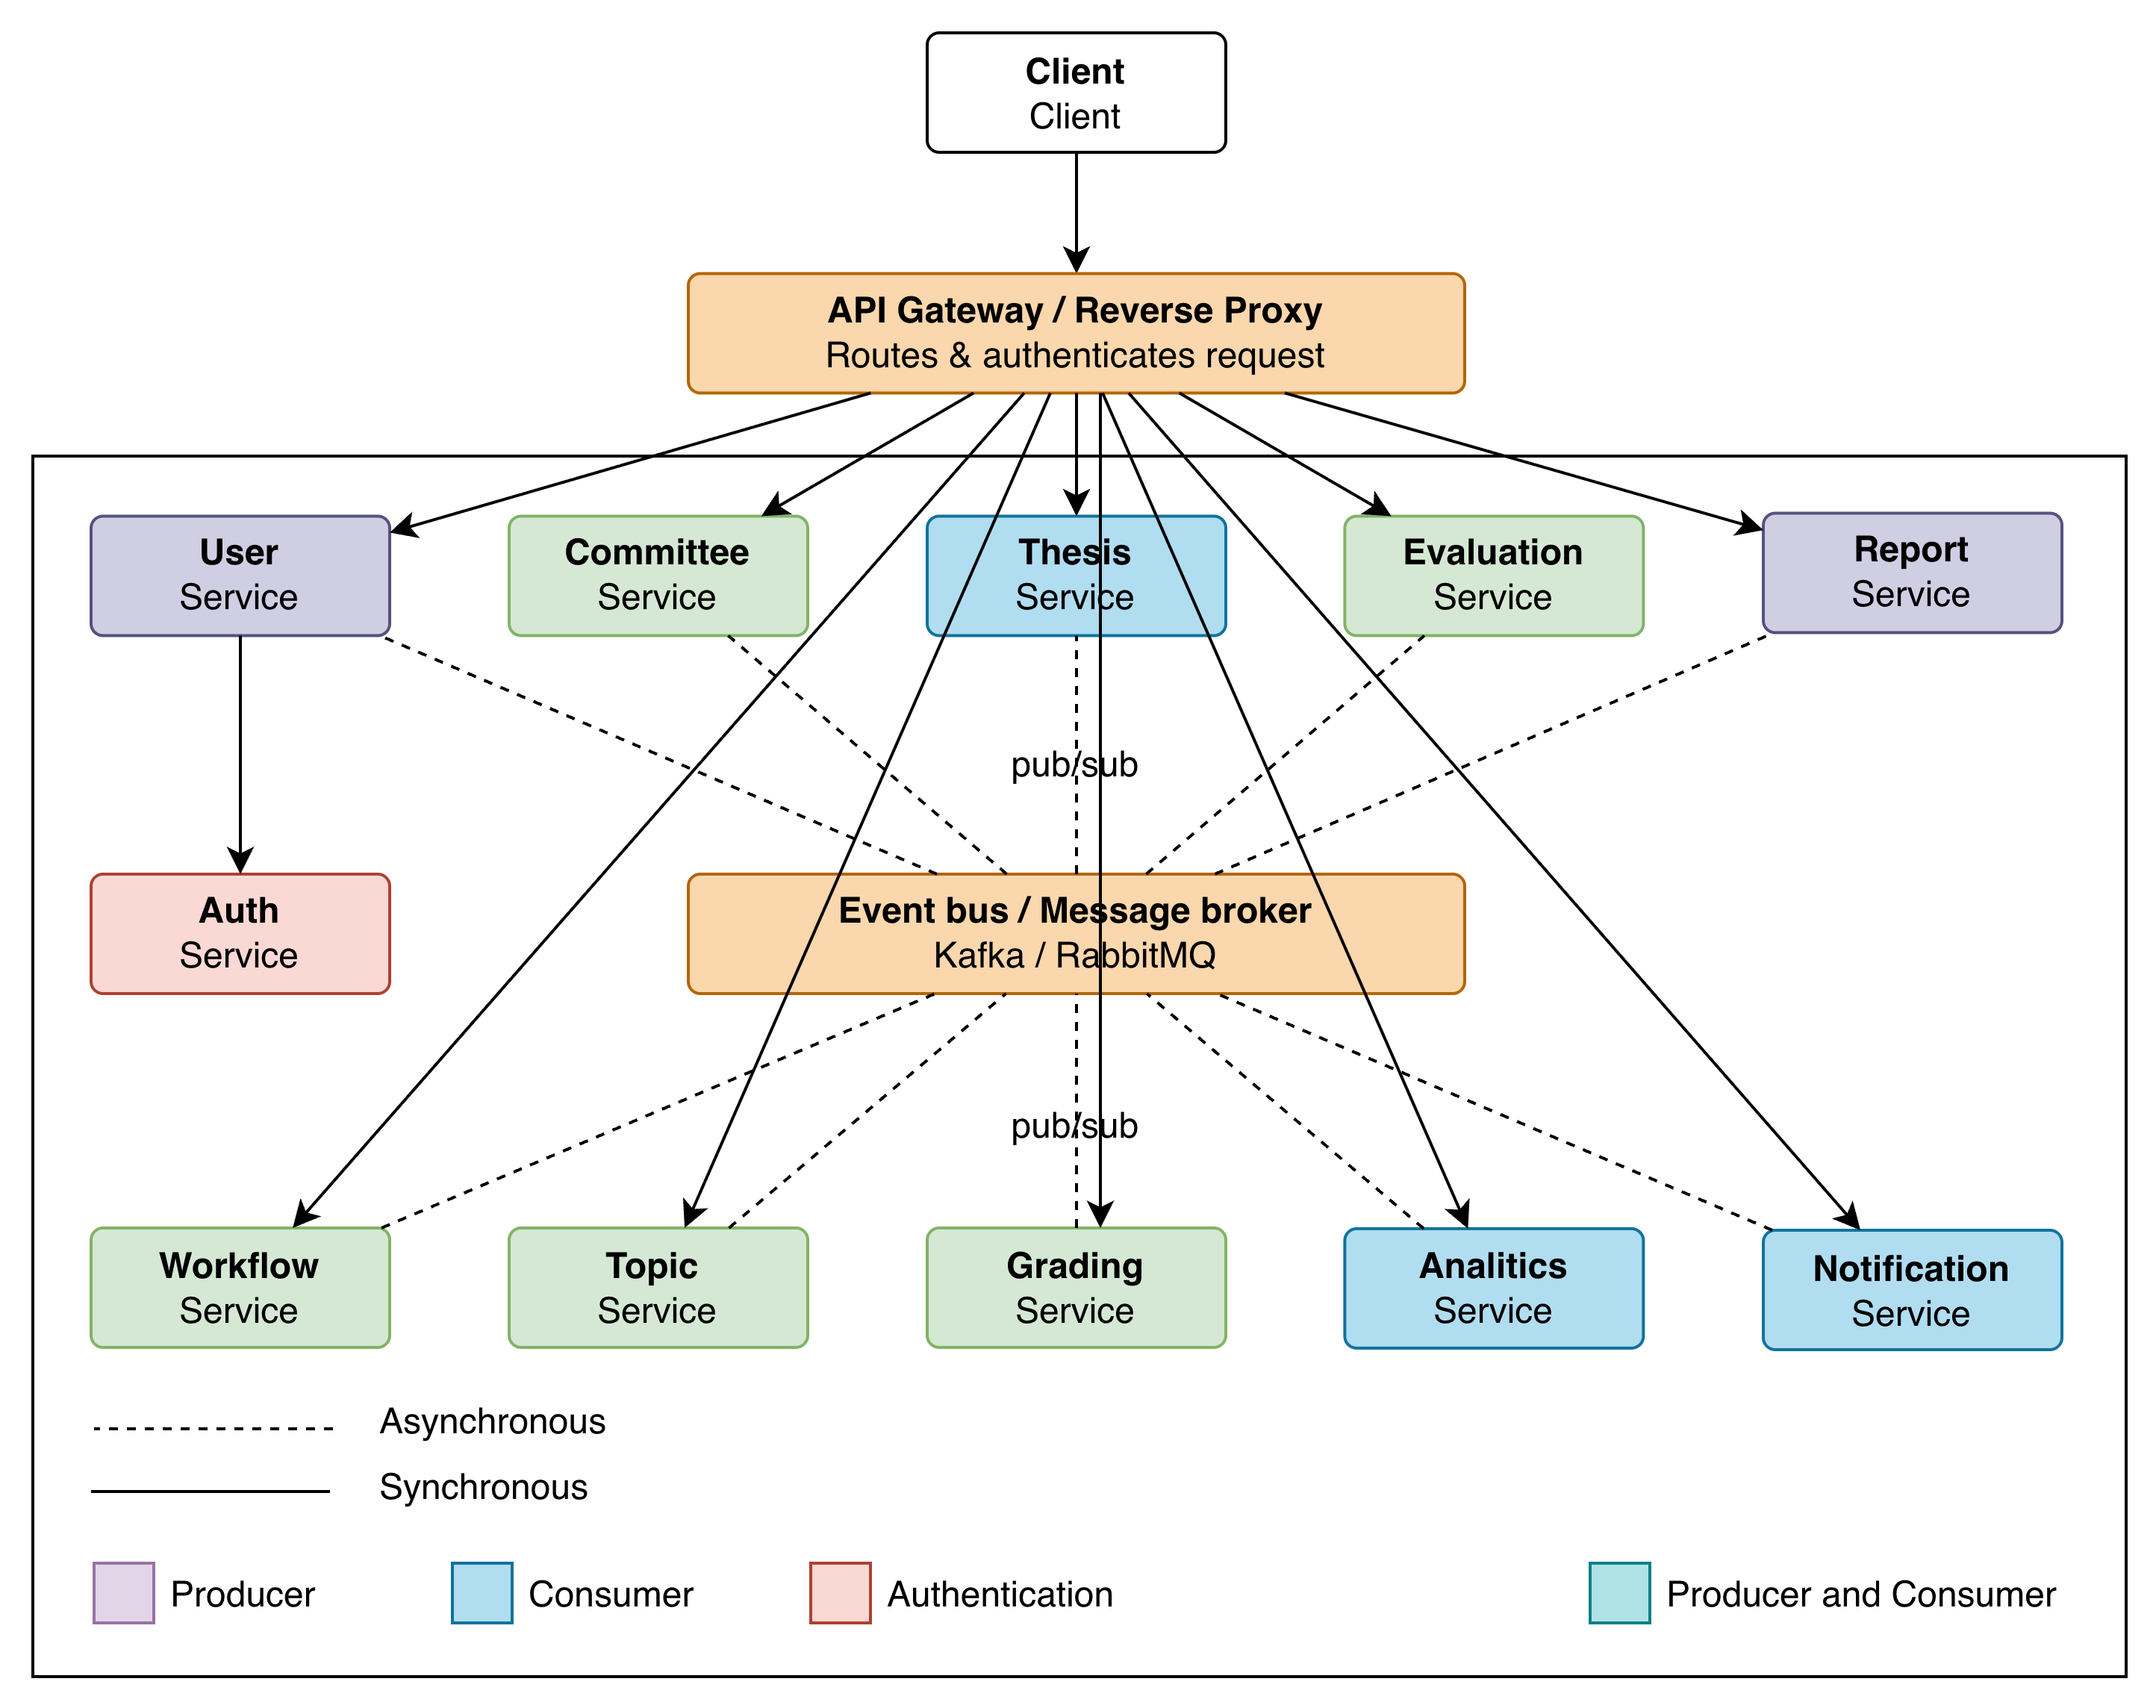
\includegraphics[width=14cm]{images/backend.png}
\caption{Микросервисүүд хоорондын харилцаа}
\label{fig:backend}
\end{figure}

% ─────────────────────────────────────────────────────────────────────
\section{Өгөгдлийн давхарга}
Энэ судалгааны хүрээнд өгөгдлийн давхаргыг дараах хоёр үндсэн хандлагын хүрээнд харьцуулан шинжилсэн:

\begin{enumerate}
\item Дундын өгөгдлийн сан: Системийн бүх сервис нэг өгөгдлийн санг хуваалцах загвар. Энэ нь транзакцийн нийцлийг хангахад хялбар боловч сервис хоорондын нягт хамаарлыг үүсгэж, бие даан хөгжүүлэх, багасгах болон томруулах боломжийг хязгаарладаг.
\item Сервис бүрт тусдаа өгөгдлийн сан: Сервис бүр өөрийн эзэмшлийн өгөгдлийн санг удирдах загвар. Энэ нь сервисийн тусгаарлалтыг дээд зэргээр хангаж, технологийн сонголтыг чөлөөтэй болгодог ч тархсан өгөгдлийн нийцлийг удирдахад нарийн төвөгтэй байдал үүсгэдэг.
\end{enumerate}

Энэхүү системд логик түвшний тусгаарлалтын шийдлийг сонгосон. Энэхүү хандлагаар бүх микросервисүүд нэг PostgreSQL инстанс дээр ажиллах боловч сервис бүр өөрийн тусдаа өгөгдлийн схемийг эзэмшинэ. Сервисүүд хоорондоо өгөгдлийн сангийн түвшинд шууд холбоос (Foreign Key) үүсгэхгүй бөгөөд зөвхөн ID-аар референц хийнэ. Ингэснээр физик түвшинд нөөцийг оновчтой удирдаж, засвар үйлчилгээг хялбарчлахын зэрэгцээ логик түвшинд микро- сервисийн бие даасан байдлын зарчмыг хадгалж байгаа юм.

\subsection{Өгөгдлийн загварчлал}

Домейнд суурилсан зохиомжийн (DDD) дагуу системийн өгөгдлийн бүтцийг Хязгаарлагдсан контекстэд хувааж, гол объект буюу \textit{Entity}-нүүдийн харилцааг тодорхойлсон (Зураг \ref{fig:domain_er}). 

Микросервис архитектурын үед өгөгдлийн сангууд тусгаарлагдмал байдаг тул олон сервисүүдийн түвшинд өгөгдлийн нэгдмэл байдлыг хангах нь гол сорилт болдог. Уламжлалт тархсан транзакшн нь системийн гүйцэтгэлд сөрөг нөлөөтэй тул энэхүү судалгаанд Eventual Consistency (Аажмын нийцэл) зарчмыг баримталсан. Өгөгдлийн нийцлийг хангахын тулд дараах хоёр үлгэр загварыг ашиглахаар загварчлав:

\begin{itemize}
\item Saga үлгэр загвар \cite{garcia1987saga}: Олон сервисийг дамжсан транзакшнийг бие даасан дэд транзакшнууд болгон хувааж, алдаа гарсан тохиолдолд нөхөн гүйцэтгэх транзакшний логикоор өгөгдлийг буцаах эсвэл засах замаар нийцлийг хангана.
\item Outbox үлгэр загвар: Сервис өөрийн өгөгдлийг шинэчлэх болон холбогдох үзэгдлийг илгээх үйлдлийг нэг атомик транзакшнд багтааснаар мэдээлэл гээгдэх эрсдэлээс сэргийлнэ.
\end{itemize}

\begin{figure}[H]
\centering
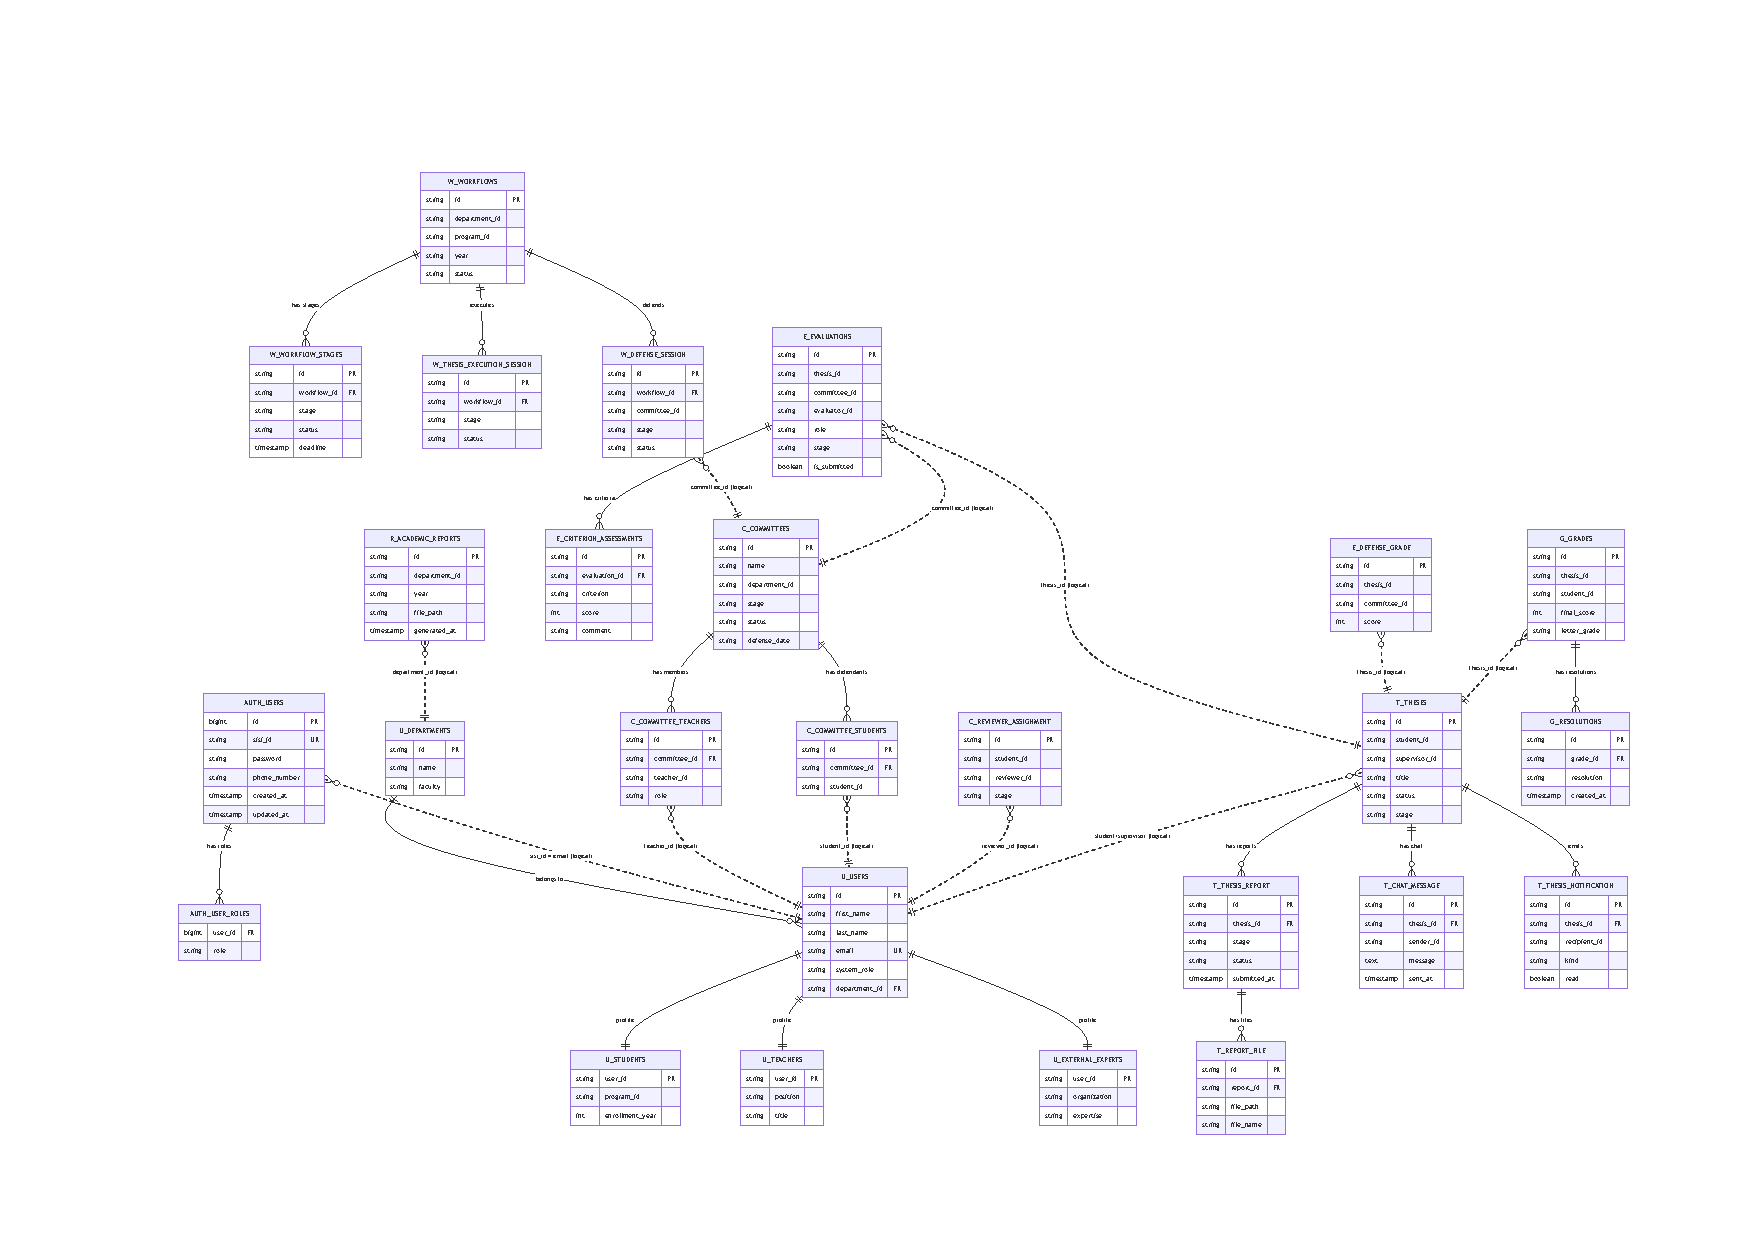
\includegraphics[width=18cm]{images/erd.pdf}
\caption{Системийн ER диаграмм}
\label{fig:domain_er}
\end{figure}

\section{Бүлгийн дүгнэлт}

Дээр тодорхойлсон Frontend (MFE), Backend (Microservices) болон холболтын давхаргууд нь нэгдсэн систем байдлаар ажиллахдаа дараах суурь зарчмуудыг баримтална:

\begin{enumerate}
\item Бие даасан хариуцлага: MFE модуль болон backend сервис бүр зөвхөн өөрийн домейны хариуцлагыг хүлээнэ.
\item API-First хандлага: Давхарга хоорондын харилцаа нь зөвхөн баримтжуулсан API гэрээ дээр үндэслэгдэнэ. Энэ нь модулиудыг хоорондоо сул холбоотой байх нөхцөлийг бүрдүүлнэ.
\item Бие даасан байршуулалт: Сервис болон MFE бүр бусдаасаа хамааралгүйгээр шинэчлэгдэх, өргөжих боломжтой байна.
\item Технологийн уян хатан байдал: Модуль бүр өөрийн домейны онцлогт тохирсон технологийн сонголт хийх боломжийг архитектурын хувьд нээлттэй үлдээв.
\end{enumerate}

\begin{figure}[H]
\centering
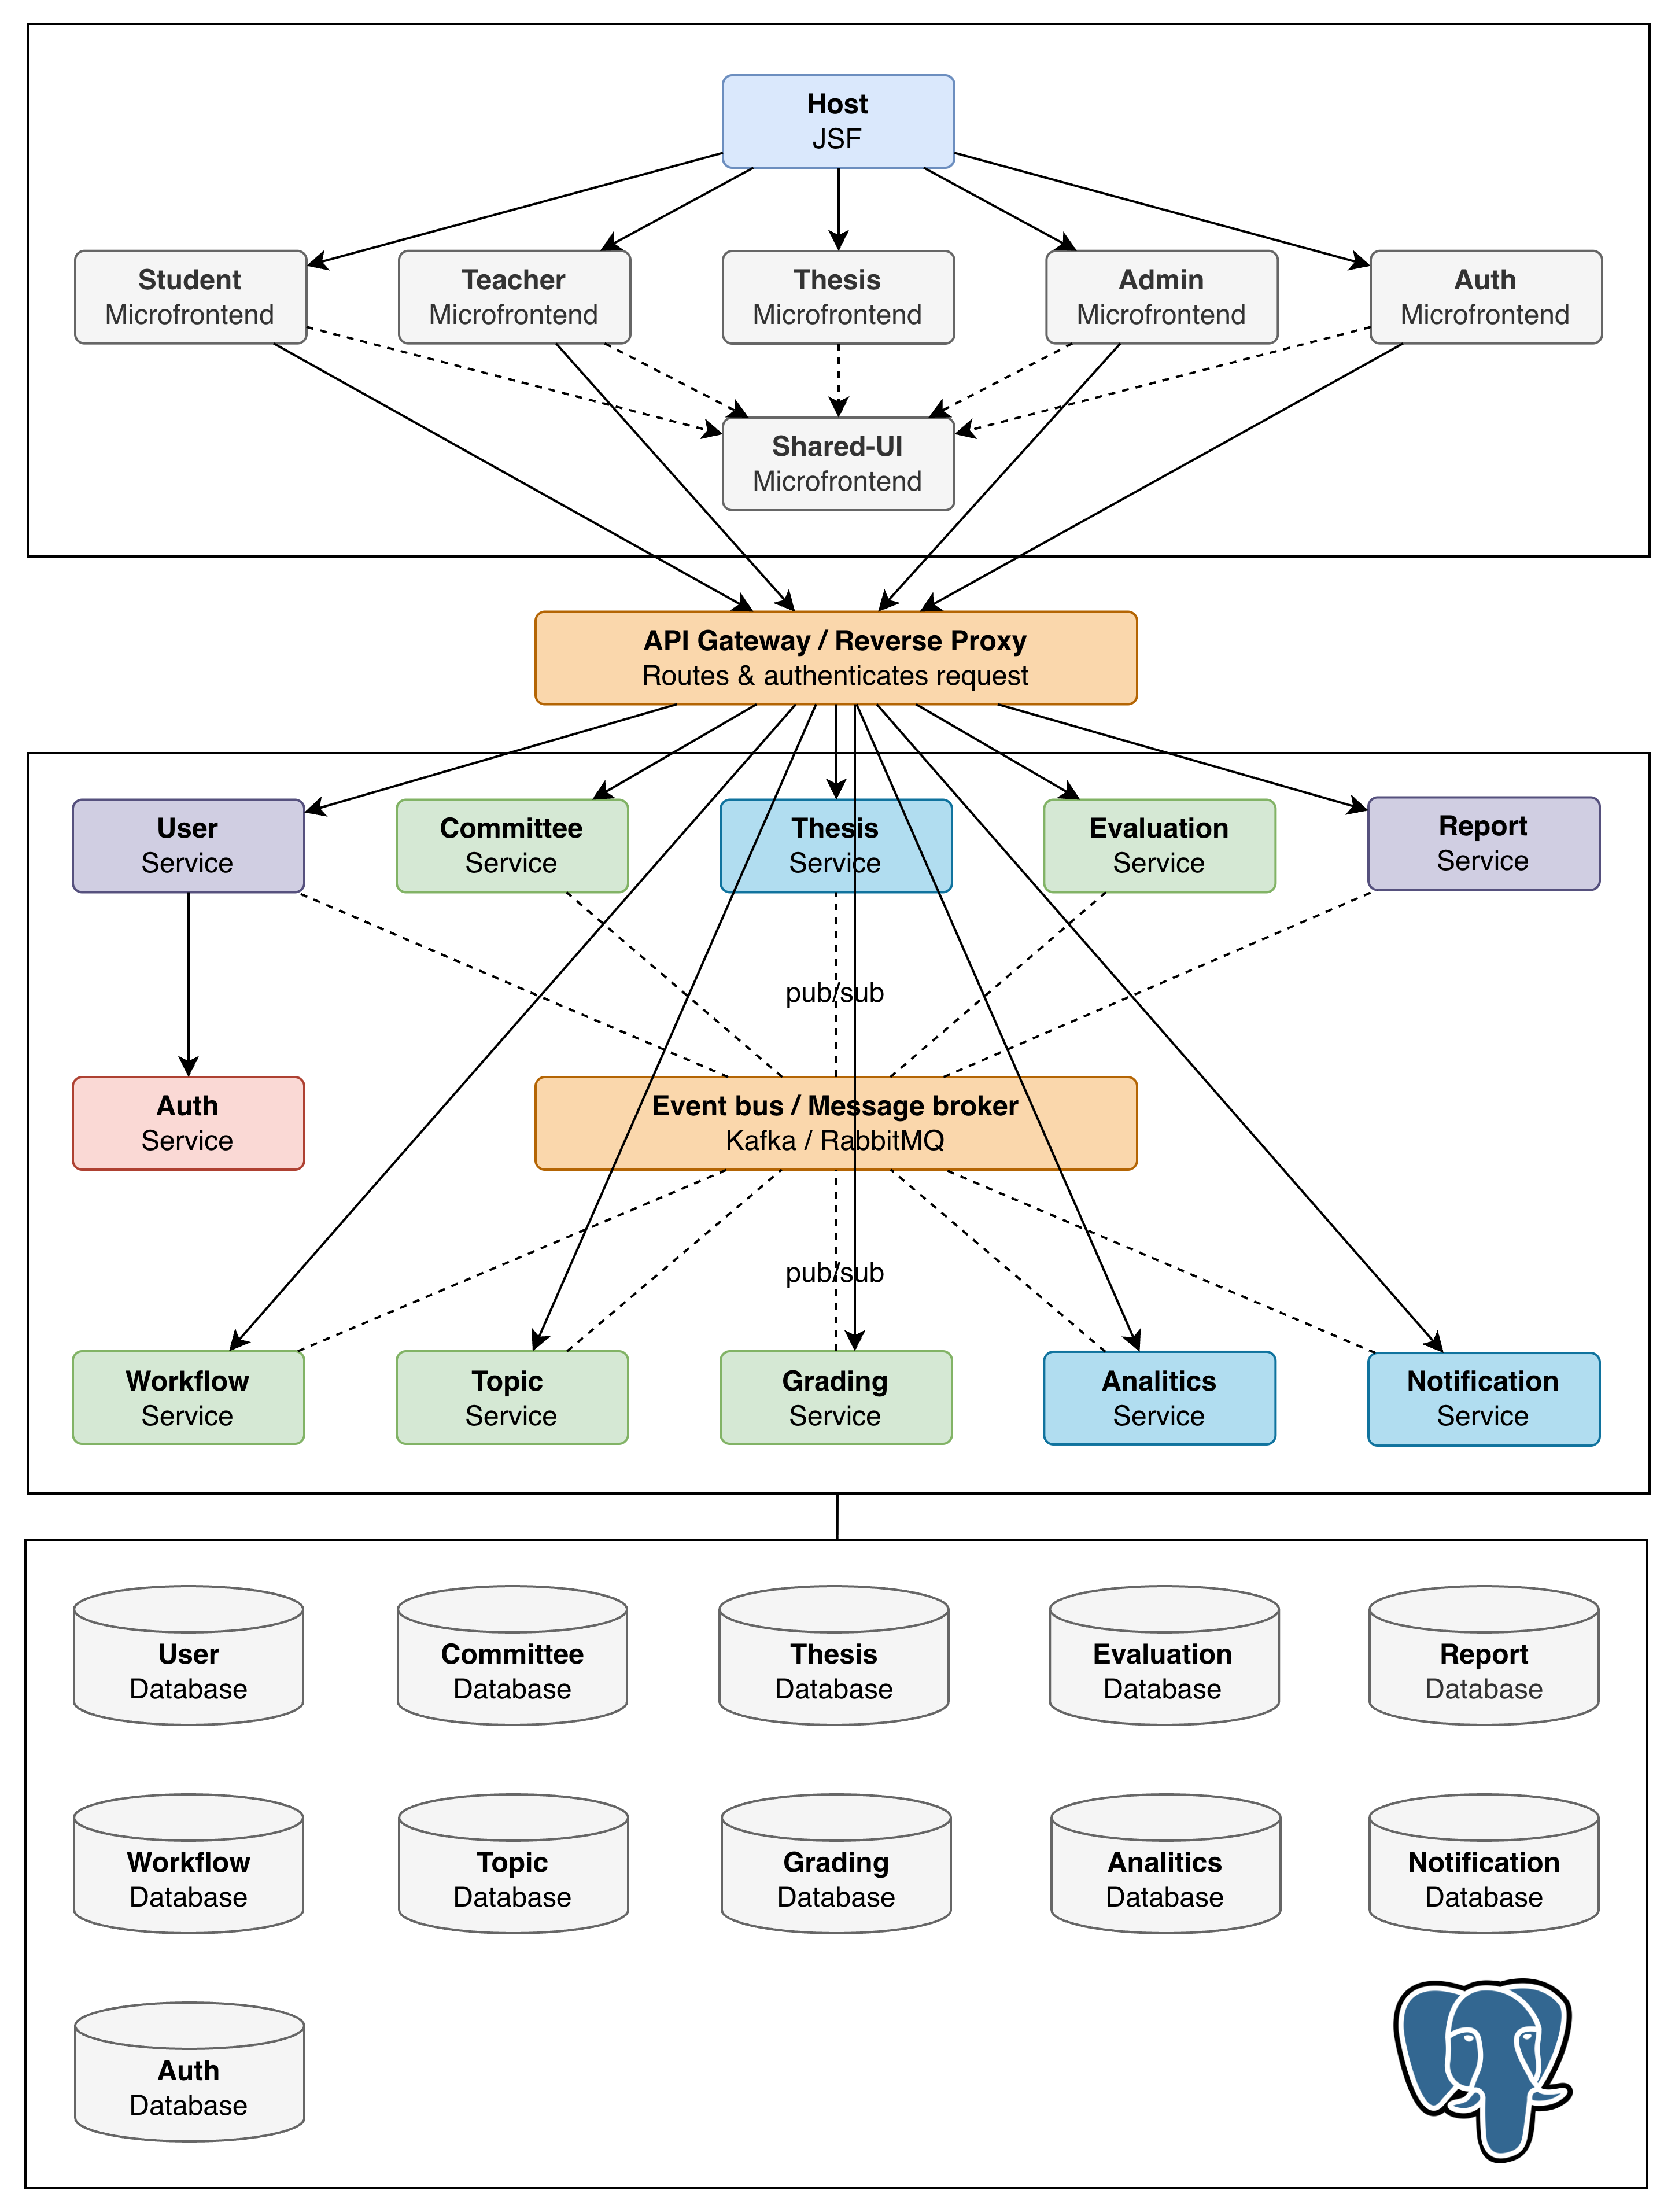
\includegraphics[width=14cm]{images/arch_tech.png}
\caption{Системийн бүрэн архитектурын нэгдсэн бүдүүвч}
\label{fig:full_architecture}
\end{figure}

Энэ бүлэгт тодорхойлсон архитектурын загварчлал болон шийдвэрүүд нь дараагийн бүлэгт авч үзэх практик хэрэгжүүлэлт, технологийн туршилтын суурь болох юм.
